\section{Biología ``quo Vadis'' \texorpdfstring{$^\dagger$}{}}
 
\let\thefootnote\relax\footnotetext{$\dagger$ \textit{quo Vadis}: del latín ``¿A dónde vas?''}
\begin{figure}[tb]
  \centering
  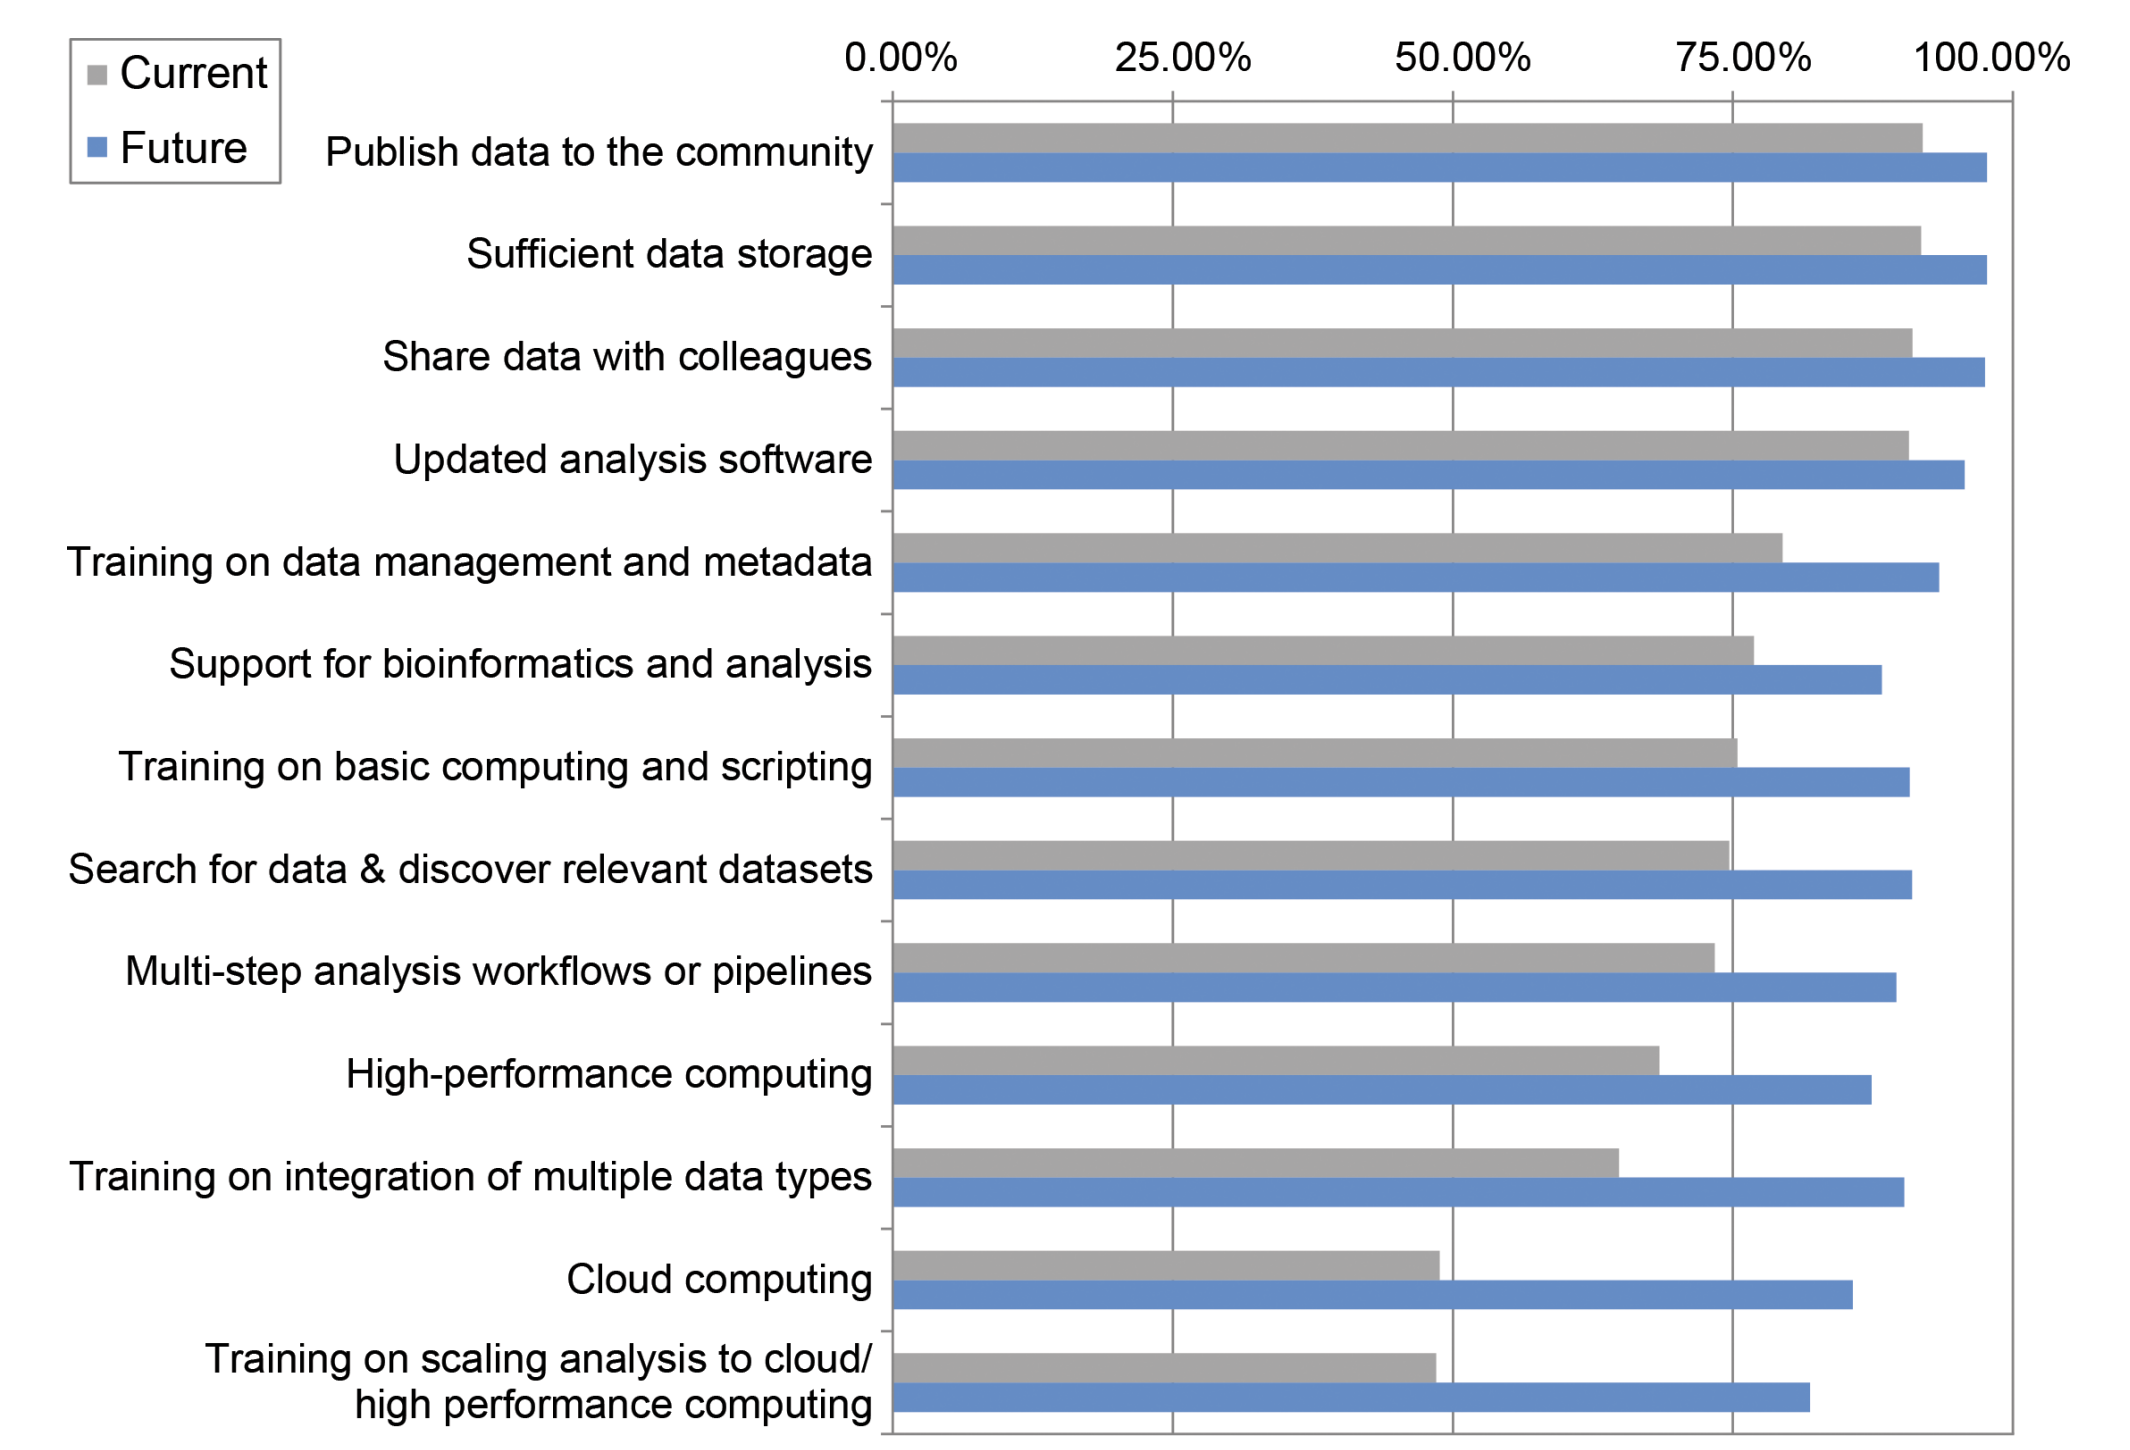
\includegraphics[width=0.8\columnwidth]{images/survey.png}
  \caption{
      (\textit{Figura en inglés})
      Necesidades computacionales actuales y futuras identificadas en una encuesta realizada a cientos de investigadores.
      Noten que las necesidades futuras son siempre mayores que las actuales, en algunos casos muy marcadamente.
      Fuente \cite{baroneUnmetNeedsAnalyzing2017}}
  \label{fig:survey}
\end{figure}
 
Como se mencionó al comienzo, es imposible abarcar en un documento tan breve el desarrollo de una ciencia tan amplia como la Biología.
Por ello, inevitablemente, se han quedado fuera muchas otras disciplinas que son ejemplos de la profunda interrelación entre la Computación y esta rama de la ciencia.
Entre ellas podemos mencionar a las Neurociencias, la Biología Celular, la Fisiología, la Ecología y otras que se han beneficiado, por ejemplo, del desarrollo de las tecnologías de imágenes digitales y su procesamiento.
Desde imágenes satelitales que son empleadas para evaluar la progresión de un daño ecológico o los patrones de migración de especies amenazadas \cite{kwokEcologyRemotesensingRevolution2018}, hasta el entrenamiento de redes neuronales para el temprano diagnóstico de cáncer a partir de imágenes de muestras de tejido \cite{mohammadzadehAdvancesOptimalDetection2015}.
Otras como la Bioacústica y la Biofísica se han beneficiado grandemente del desarrollo del procesamiento de señales en general.
Por ejemplo, investigadores graban el sonido ambiente en los hábitats y luego lo procesan para estimar realizar el tamaño de poblaciones de diversos animales simultáneamente.
La identificación de las especies y la cantidad de individuos se puede estimar mediante \textit{Machine Learning} \cite{kahlBirdNETDeepLearning2021}.
Al igual que las ómicas, todas estas disciplinas vienen acompañada de grandes acumulaciones de datos.
 
Por otro lado, otro fenómeno significativo es la democratización del acceso a las tecnologías de la información.
Movimientos como el $\textit{Open Software}$ y $\textit{Open Hardware}$ han abierto un sinfín de nuevas posibilidades \cite{ravindranHowDIYTechnologies2020}, particularmente en los países en vías de desarrollo.
Hoy en día es posible fabricar ``en casa'', usando tecnologías como la impresión 3D y microcontroladores, los sensores e instrumentos necesarios para la investigación.
Esto no solo puede abaratar los costos, también permite que los investigadores diseñen los artefactos acorde a sus necesidades más particulares.
Nunca ha habido más flexibilidad en el aspecto experimental.

La Biología se encuentra hoy en una posición muy diferente si es comparada con los comienzos de este siglo.
La disponibilidad de grandes cantidades de datos ha aumentado considerablemente la necesidad de introducir nuevas habilidades en el currículum de los estudiantes e investigadores.
En una encuesta reciente realizada a varios cientos de investigadores de alto perfíl, se identificó como una de las principales áreas a priorizar, el entrenamiento de las nuevas generaciones en las habilidades requeridas para la manipulación, publicación y procesamiento de datos \cite{baroneUnmetNeedsAnalyzing2017} (Figure \ref{fig:survey}).
Esto avizora un futuro donde un sólido entrenamiento en computación no sea ya una habilidad excepcional, sino, esperada para un graduado de una especialidad biológica.
Como mencionamos anteriormente, no existen herramientas propias de una disciplina, ni herramientas que estén fuera de su interés. Existen problemas fundamentales, y cada disciplina deberá considerar suyas todas aquellas que les permitan abordar los propios, la Biología no es excepción.
 
\rightline{$\blacksquare$}
 

